

\title{Popper Example: A Random Sample}
\author{
        Quincy Wofford \\
}
\date{\today}

\documentclass[12pt]{article}
\usepackage{graphicx}

\begin{document}
\maketitle

\begin{abstract}
Seven samples are drawn from a node over N iterations, where N is defined in the simulations.sh file. In this paper, a histogram of N samples is shown. The samples are harvested from a csv file. The column which is shown here is exclusively from the column called "sample".
\end{abstract}

\section*{Introduction}
What follows is a convincing argument that a simple experiment can be simply popperized.
\section*{Method}
This is a popperized project. The ./setup.sh script will generally prepare the execution environment for a particular set of resource. In this case, setup.sh simply complains if the experiment is run on the Wheeler head node. 
\paragraph{}
The main workload for this experiment is defined in run/simulation.sh, and some requisite post-processing is handled in the pipeline with post-run/concatenate\_output.sh. A detailed description of this experiment is below:
\begin{verbatim}
./run/simulation.sh
\end{verbatim}
Some post processing is required to make the results useful.
The function of this file is explained below:
\begin{enumerate}
\item Loops over N iterations (5 is default)
\item For each iteration, generate a new csv file whose filename is the name of the node it runs on, concatenated with a random 32 character string, and the extension csv.
\item For each iteration, a for loop is called M times (100 is default)
\item 7 random samples are drawn N*M times. The samples come from /dev/urandom, which may or may not be uniformly distributed. The M samples are appended to the N csv files.
\item All files are collected under the results/job\_output/ directory.
\item The post-run script cat's all the files in results/job\_output/ directory and places a result.csv file in the results/ directory
\item The validation step of this pipeline generates a histogram of one column from the concatenated csv file. The title of the column whose histogram is shown is "sample"
\item The figure is placed in validation/, and then builds this \LaTeX document using the same PNG file output
\end{enumerate}

\paragraph{}
After the post-run.sh script finishes, the ./teardown.sh script is executed. This script is generally meant to clean up after infrastructure configuration details regarding ./setup.sh. In this case however, the teardown script shames the user for running on the Wheeler head node or congratulates them for not doing so.
\section*{Results}
This section is broken down into two sections: one for the results of the random sample experiment itself,  the second for the logs, errors, and outputs of the Popper pipeline itself.
\subsection*{Experiment Results}
The results of the experiment itself may be viewed according to your needs. In this case, results are viewed in this \LaTeX document. The only thing about this document that changes after running the popper pipeline is the histogram seen below. It's easy to imagine scenarios where numeric results and many figures are stored in a file, then inserted into the paper. Some care when writing the paper must be taken to include the falsifiability goals. Clearly stating the implication, experiment result, with case statements to break down whether the newly generated paper does or does not violate evaluation thresholds.

\begin{center}
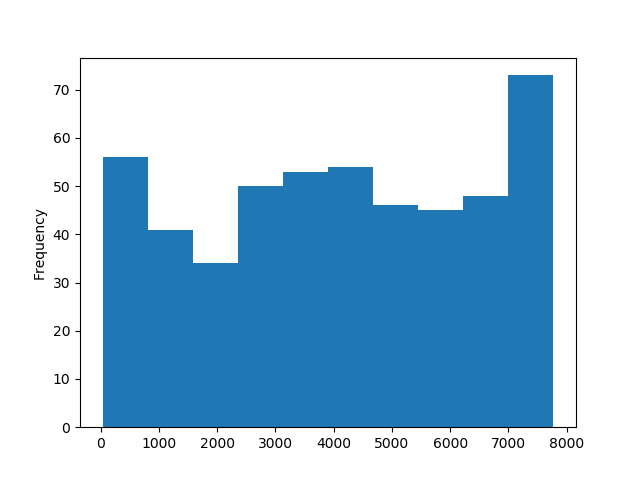
\includegraphics[scale=0.5]{../all_sample_hist.png} 
\end{center}

\subsection*{Pipeline Results}
The Popper pipeline generates results from its execution which may be found in your experiment folder under the popper/ directory. This is where you will find my setup and teardown notes, for instance. The popper pipeline will export error files and output files, so you'll want to check both to determine if your run was successful, or where your run failed.

\paragraph{}
Perhaps the most useful tool in creating my own pipeline was the experiment flowchart which popper automatically generates. I based my flowchart and this pipeline structure off the quiho, single-node, experiment. The flowchart generated for this pipeline is below:
\begin{center}
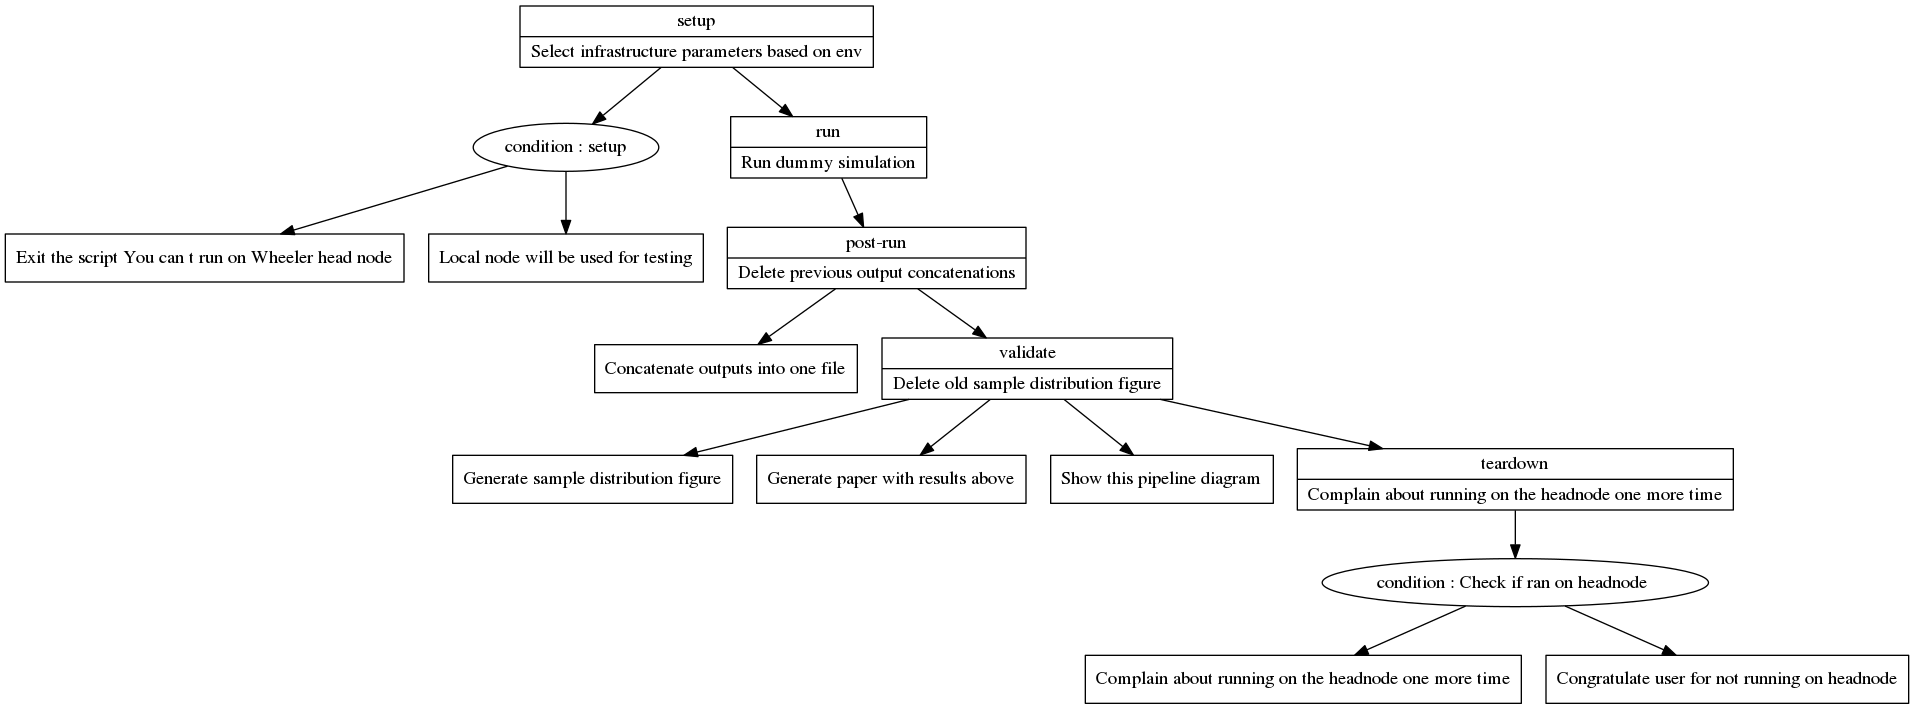
\includegraphics[scale=0.2]{../../wf.png}
\end{center}
\section*{Future work}
Next steps may be completed in any order, and probably include but are not limited to:
\begin{itemize}
\item Incorporate jupyter-notebooks in analysis. A small template/sample of such a notebook is included in the top-level analysis directory. Perhaps testing that this distribution is indeed normal and creating a separate paper about that result would be appropriate, | \textbf{Chris}
\item Parallelize the pipeline. This simulation is embarrassingly parallel, and requires no software dependencies. | \textbf{Quincy}
\item Alter the setup/teardown scripts to configure and deploy a Singularity/CharlieCloud image on Wheeler, in parallel, and collect results of simulation.sh or some other simulation | \textbf{Quincy}
\item Replace simulation.sh with BSP distribution simulator. | \textbf{Keira}
\item Implement a continuous integration pipeline | \textbf{Quincy}
\item Experiment with analysis live analysis notebooks such as the hosted solution, Binder. | \textbf{Quincy}
\end{itemize}

\section*{Conclusion}
This experiment is Popperized. It takes some time to do, but it is a one-time time investment on the order of hours which will formalize our approach to reproducibility and enable us to gracefully deploy on many infrastructures.


\end{document}

